\documentclass[a4paper,11.5pt,]{article}
\usepackage[utf8]{inputenc}
\usepackage[T1]{fontenc,url}
\usepackage[english,]{babel}
\usepackage{blindtext}
\usepackage{natbib}
\usepackage{gensymb}
\usepackage{amsmath}
\usepackage{changepage}
\usepackage{amssymb}
\usepackage{commath}
\usepackage{physics}
\usepackage{multicol}
\usepackage{float}
\usepackage{listings}
\usepackage{graphicx}
\usepackage{hyperref}
\usepackage{svg}
\usepackage{wrapfig}

\newenvironment{Figure}
  {\par\medskip\noindent\minipage{\linewidth}}
  {\endminipage\par\medskip}

\usepackage{multicol}
%\setlength{\columnsep}{1cm}

\usepackage{geometry}
 \geometry{
 a4paper,
 total={170mm,257mm},
 textheight =  592mm,
 left=20mm,
 right=20mm,
 tmargin=20mm,
 bmargin=20mm
 }
 \setlength{\columnsep}{20pt}
          

 \title{Stellar Spectra A. - Basic Line Formation\\
 AST4310}
 \date{\normalsize{14. September 2018} }
 \author{\textsc{\small{Metin San}}}
 
 
\begin{document}

\maketitle
\begin{center}
\textsc{Introduction}
\end{center}


\begin{adjustwidth}{1cm}{1cm}

Spectral lines in stellar spectra make out the foundation of astrophysics. They provide a wealth of knowledge about the studied object and are therefore one of the most valuable sources of information to an astrophysicist. In order to get an understanding of spectral lines we will follow the work of Cecilia Payne and Marcel Minnaert which are some of the early pioneers of spectral astronomy. The report is split into two parts. The first part considers Saha-Boltzmann modeling with Cecilia Payne, while the second part deals with Fraunhofer lines and their strenghts with Marcel Minnaert.
\end{adjustwidth}
\begin{multicols}{2}

\begin{center}
\textsc{1. The Boltzmann and Saha laws}
\end{center}
Cecilia Payne (1900 - 1979) was a British-American astronomer and astrophysicist famous for showing that most stars are made of mainly hydrogen and helium. She applied the Saha distribution which was newly derived to stellar spectra. With this she was able to show that the empirical Harvard classification primarily represented a temperature scale.

In thermodynamical equilibrium, the equipartition laws Saha and Boltzmann describe the division of particles of a specific element. With the temperature as the only major parameter these laws show us how the different ionization stages and discrete energy levels of a specific element are distributed.

\begin{center}
1.1 \textit{Boltzmann distribution}
\end{center}
The Boltzmann distribution deals with the energy levels and is given by
\begin{equation}\label{eq:1}
    \frac{n_{r,s}}{N_r} = \frac{g_{r,s}}{U_r} e^{-\chi_{r,s}/kT},
\end{equation}
where $n_{r,s}$ is the number density (also called level population) and $g_{r,s}$ the statistical weight of the level $(r,s)$ where $r$ is the ionization stage, and $s$ is the state or level. $N_r = \sum_3 n_{r,s}$ is the total particle density over all levels of ionization. $\chi_{r,t}$ is the excitation energy measured from the ground state ($r,s=1$). The partition function $U_r$ is defined by

\begin{equation}\label{eq:2}
    U_r = \sum_s g_{r,s} e^{-\chi_{r,s}/kT}.
\end{equation}

\begin{center}
1.2 \textit{Strength ratio of $\alpha$ lines in hydrogen}
\end{center}
Payne was studying the absorption lines in stellar spectra when she made the assumption that the strength of the absorption lines scaled with the population density of the lower level of the corresponding transition. If one assumes that most of the hydrogen resides in the lower energy levels, it follows that most transitions would result in higher energy levels. The strength of the lines should therefore scale with the population density of these lower levels. We know today that this is assumption is completely correct, but stellar absorption lines do generally scale with larger lower-level populations. We will therefore proceed by assuming that Payne's assumption holds and that the scaling is linear.

This assumption allows us to estimate the strength ratios of the $\alpha$ lines of hydrogen, where $\alpha$ denotes that the excitation is from $s$ to $s+1$.  For a neutral hydrogen atom ($r = 1$), the statistical weight goes as $g_{1,s} = 2s^2$, and the excitation energy goes as $\chi_{1,s} = 13.6 (1- 1/s^2)$. The ratio between Lyman $\alpha$ ($s=1$) and Balmer $\alpha$ ($s=2$) is then given from the Boltzmann equation \eqref{eq:1} as

\begin{equation}\label{eq:3}
    \frac{n_{1,1}}{n_{1,2}} = \frac{g_{1,1}e^{-\chi_{1,1}/kT}}{g_{1,2} e^{-\chi_{1,2}/kT}},
\end{equation}
where $U_r$ and $N_r$ have canceled out. We only need to insert for $s$ and $g$ in order to compare. By using the formula in equation \eqref{eq:3} we can compute the strength ratio of the $\alpha$ lines in H I Lyman, Balmer, Paschen and Brackett series. For neutral hydrogen, the information need is tabulated in table \ref{tab:1}. Using the information in this table we find that the following strength ratios for the solar temperature of 5770 K: (Lyman $\alpha$ / Balmer $\alpha$) $\approx 2 \cdot 10^8$, (Balmer $\alpha$ / Paschen $\alpha$) $\approx $ 20, and (Balmer $\alpha$ / Brackett $\alpha$) $\approx 42$. We see that Lyman $\alpha$ line strength is enormous compared to the other lines. This is a result of the excitation energy $chi_{1,1} = 0$, making it temperature independent when computing ratios.

\begin{table}[H]
\begin{center}
\begin{tabular}{llll}
\hline
Line $\alpha$ & $s$ & $\chi_{1,s} $ {[}eV{]} & $g_{1,s}$ \\ \hline
Lyman         & 1   & 0                      & 2          \\
Balmer        & 2   & 10.20                  & 8          \\
Paschen       & 3   & 12.09                  & 18         \\
Brackett      & 4   & 12.75                  & 32         \\ \hline

\end{tabular}
\caption{Neutral hydrogen information}
\label{tab:1}
\end{center}
\end{table}





\begin{center}
1.3\textit{ Saha distribution}
\end{center}
The Saha distribution relates the ionization levels of an element in ionization equilibrium and is given by

\begin{equation}\label{eq:4}
    \frac{N_{r+1}}{N_r} = \frac{1}{N_e} \frac{2U_{r+1}}{U_r} \left( \frac{2\pi m_e k T}{h^2} \right)^{3/2} e^{-\chi_r /kT},
\end{equation}
where $m_e$ is the electron mass, $h$ is Planck's constant $N_e$ is the electron density, and $\chi_r$ is the threshold ionization energy required to ionize from stage $r$ to $r+1$.

\begin{center}
1.4\textit{ Element E (Schadeenium)}
\end{center}
We will now consider the imaginary element E, or "Schadeenium". E is a simple atom which lets us evaluate Saha-Boltzmann statistics without having to bother about complex atomic data. It has the following properties:
\begin{itemize}
    \item The statistical weight is $g_{r,s} = 1$ for all levels.
    \item For neutral E, the ionization energy is $\chi_1 = 7$ eV. For $E^+$ (ionized once) the energy is $\chi_2 = 16$ eV, and similarly $\chi_3 = 31$ eV and $\chi_4 = 51$ eV.
    \item The excitation energies increase incrementally by 1 eV: $\chi_{r,s} = s-1$ eV.
\end{itemize}

\noindent We begin by computing the partition function $U_r$ of E found in equation \eqref{eq:2}. The results is seen in figure \ref{fig:1}.

\begin{figure}[H]
	\centering
	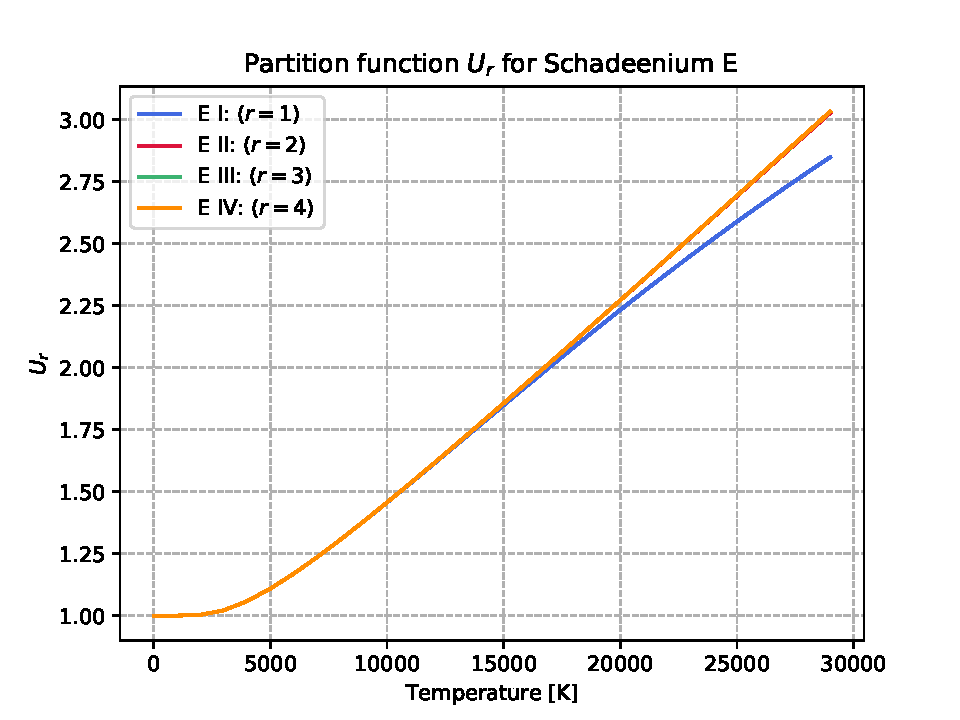
\includegraphics[width=0.5\textwidth]{figures/part_E.pdf}
	\caption{Partition function $U_r$ for the imaginary element E.}
	\label{fig:1}
\end{figure}

\noindent We find that all ionizations mostly behave the same way for temperatures below 15000 K. For higher temperatures, $U_1$ splits from the other ionizations and keeps a lower value. Generally we note that the partition function of element E is of order unity and appears to be weakly sensitive to temperature.

\begin{center}
1.4.1 \textit{ Boltzmann distribution for E}
\end{center}
With the partition function calculated, we can study the Boltzmann distribution for E. This is done by computing the boltzmann equation \eqref{eq:1} for varies levels $s$. The result can be seen in figure \ref{fig:2}.

\begin{figure}[H]
	\centering
	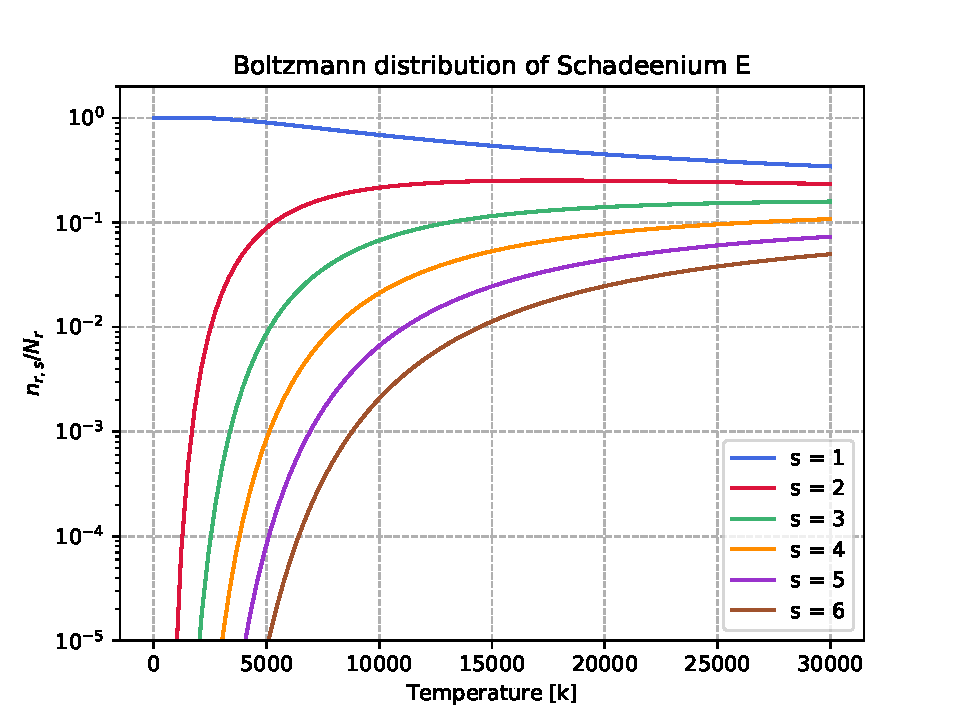
\includegraphics[width=0.5\textwidth]{figures/boltz_E.pdf}
	\caption{Boltzmann distribution of the imaginary element E.}
	\label{fig:2}
\end{figure}

\noindent By studying figure \ref{fig:2} we notice that in thermal equilibrium, for all temperatures, the ground state always has the largest population. At $T = 5000$ K we have $n_{r,s}/N_r = 0.9$ for $s = 1$ and $n_{r,s}/N_r \approx 0.009$ for $s=2$ and so on for the lower levels. We see that all these add up to unity for all temperatures, which is a results off the scaling by $N_r$. We can conclude that the lowest levels are the most important ones which is a result of the rapid decay of the Boltzmann factor $e^{-\chi_{r,s}/kT}$. This can also explain the insensitivity of $U_r$ to temperature. 

\begin{center}
14.2\textit{ Saha distribution for E}
\end{center}

We will now study the Saha distribution of the element E. By computing the saha equation \eqref{eq:4} for varying ionizations we obtain the results seen in figure \ref{fig:3}. Since this is a normalized distribution in the same way as the Boltzmann distribution, the ionizations always add up to one. We also notice that for 

\begin{figure}[H]
	\centering
	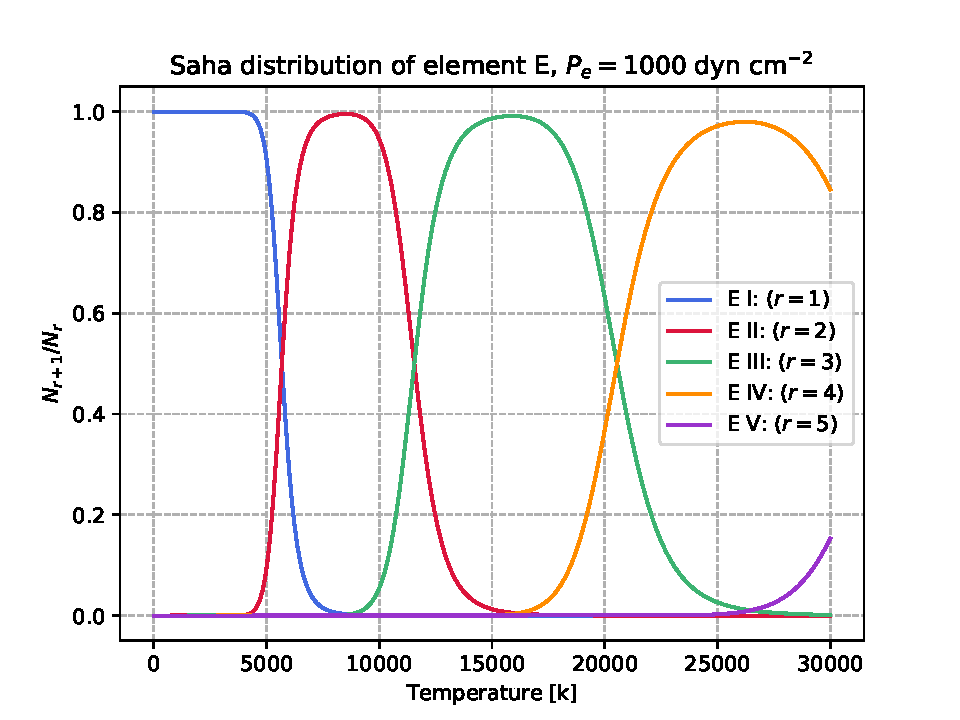
\includegraphics[width=0.5\textwidth]{figures/saha_E.pdf}
	\caption{Saha distribution of the imaginary element E with an electron pressure of $P = 1000$ dyn cm$^{-2}$ .}
	\label{fig:3}
\end{figure}


\end{multicols}
\end{document}